\section{Case Study}

\begin{frame}[plain]
	\frametitle{\polu}
	\begin{figure}
		\centering
			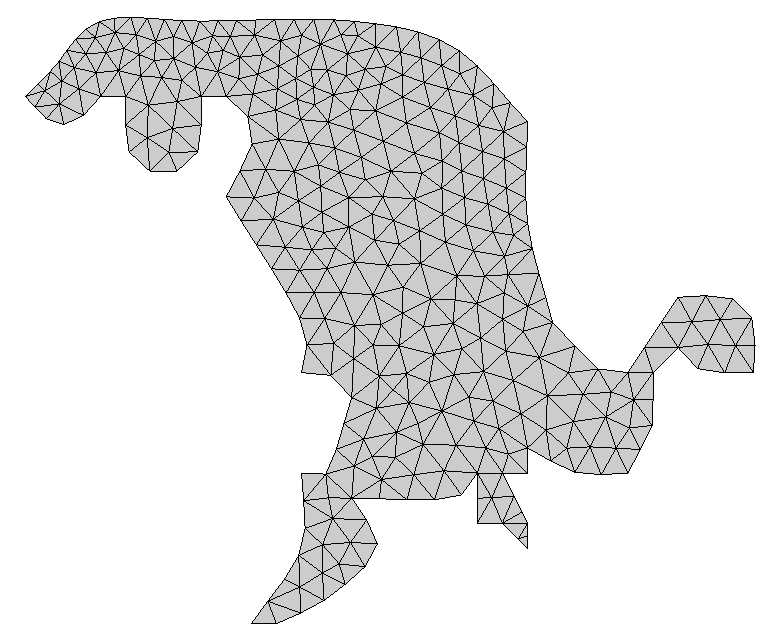
\includegraphics[width=.6\textwidth]{images/foz_msh.png}
	\end{figure}
	\pause
	\begin{description}
		\item [\computeflux] computes the flux transfered through the edges;
		\item [\update] uses the compute fluxes to update the value in each cell;
	\end{description}
\end{frame}

\begin{frame}
	\frametitle{Environmental Setup}

	\begin{block}{SeARCH Group Hex}
		\begin{description}
			\item [] Intel\textsuperscript{\textregistered} Xeon\textsuperscript{\textregistered} X5650
			\item [2] processors per node;
			\item [6] cores per processor;
			\item [-] Intel\textsuperscript{\textregistered} HyperThreading Technology;
			\item [2.66] GHz clock frequency;
			\item [12 to 48] GB of RAM;
			\item [Tesla M2070]
			\begin{description}
				\item [1] Tesla CPU;
				\item [448] CUDA cores;
				% \item [1.15] GHz clock frequency;
				\item [515] Gflops peak (double);
				\item [6] GB dedicated memory;
				\item [148] GB/sec memory bandwidth;
			\end{description}
		\end{description}
	\end{block}
\end{frame}

\begin{frame}{Methodology}
	\begin{itemize}
		\vfill
		\item Limited execution: 5000 iterations;
		\vfill
		\item Median of 10 executions;
		\vfill
		\item 62 MB test case;
		\vfill
		\item Measurements focused on final speedups;
		\vfill
	\end{itemize}
\end{frame}